\documentclass[10pt,mathserif]{beamer}

\usepackage{graphicx,amsmath,amssymb,tikz,psfrag,subfigure,bm,cancel}

\input defs.tex

%% formatting

\mode<presentation>
{
\usetheme{default}
}
\setbeamertemplate{navigation symbols}{}
\usecolortheme[rgb={0,0,0}]{structure}
\setbeamertemplate{itemize subitem}{--}
\setbeamertemplate{frametitle} {
	\begin{center}
	  {\large\bf \insertframetitle}
	\end{center}
}

\AtBeginSection[] 
{ 
	\begin{frame}<beamer> 
		\frametitle{Outline} 
		\tableofcontents[currentsection,currentsubsection] 
	\end{frame} 
} 

%% begin presentation

\title{\large \bfseries Markov and hidden Markov models}

\author{Jiali Lin\\[3ex]
Virginia Tech}

\date{\today}

\begin{document}

\frame{
\thispagestyle{empty}
\titlepage
}

\section{Introduction}
\begin{frame}{Markov Chains}
\begin{itemize}
    \item First order Markov chain
    \begin{equation*}
        p(x_{1:T}) = p(x_1)\prod_{t=2}^Tp(x_t |x_{t-1})
    \end{equation*}
    \begin{figure}[h]
    \centering
    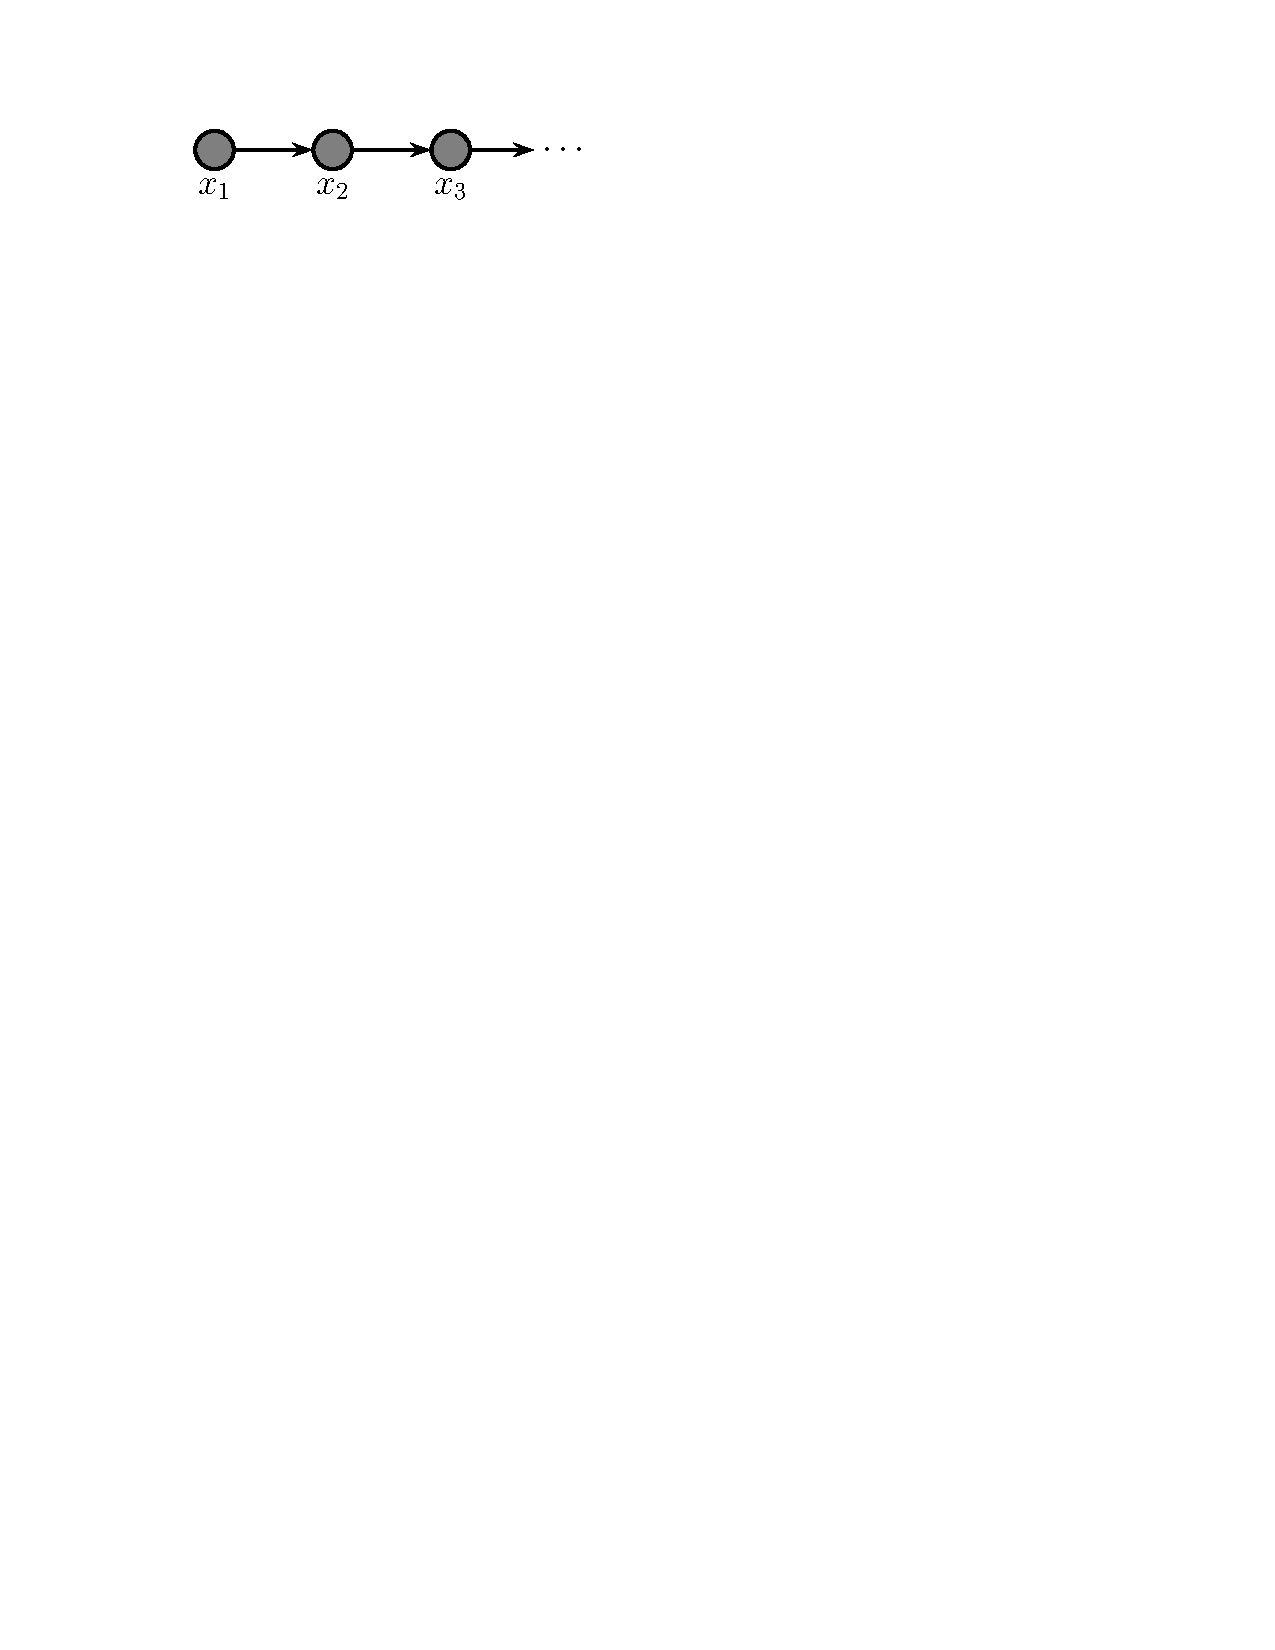
\includegraphics[width=0.3\textwidth]{markovChain1xCropped}
    \end{figure}

    \item Second order Markov chain
    \begin{equation*}
        p(x_{1:T}) = p(x_1)p(x_2)\prod_{t=3}^Tp(x_t |x_{t-1,t-2})
    \end{equation*}
    
    \begin{figure}[h]
    \centering
    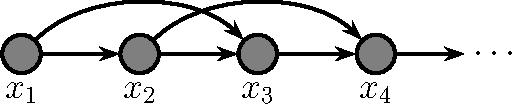
\includegraphics[width=0.3\textwidth]{markovChain2}
    \end{figure}
\end{itemize}  
\end{frame}

\begin{frame}{State Diagrams}
\begin{itemize}
    \item \textbf{State Transition Matrix}:  $A_{ij} = p(x_t = j | x_{t - 1} = i)$
    \item State Transition Diagram: One node per discrete state.
\end{itemize}

\begin{figure}
\centering
\subfigure[]{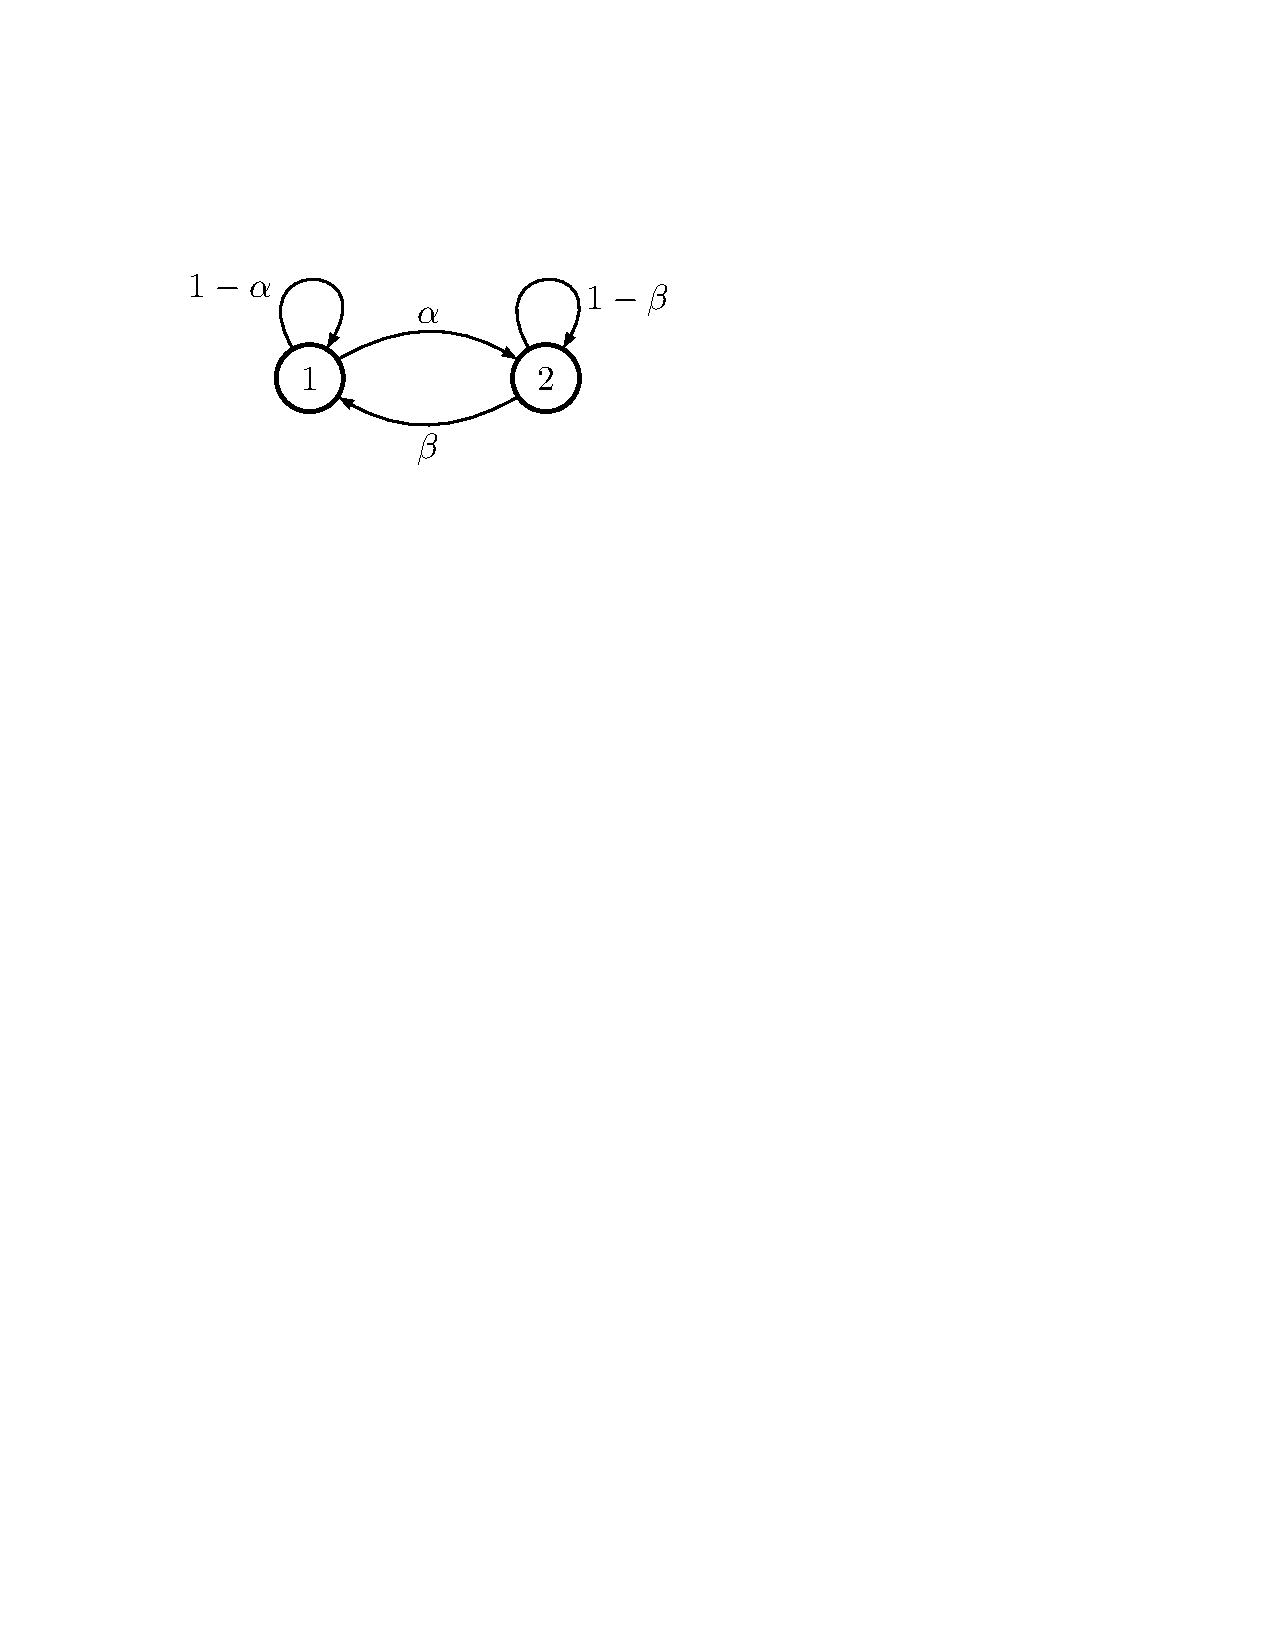
\includegraphics[width=40mm]{MC2state}}
\subfigure[]{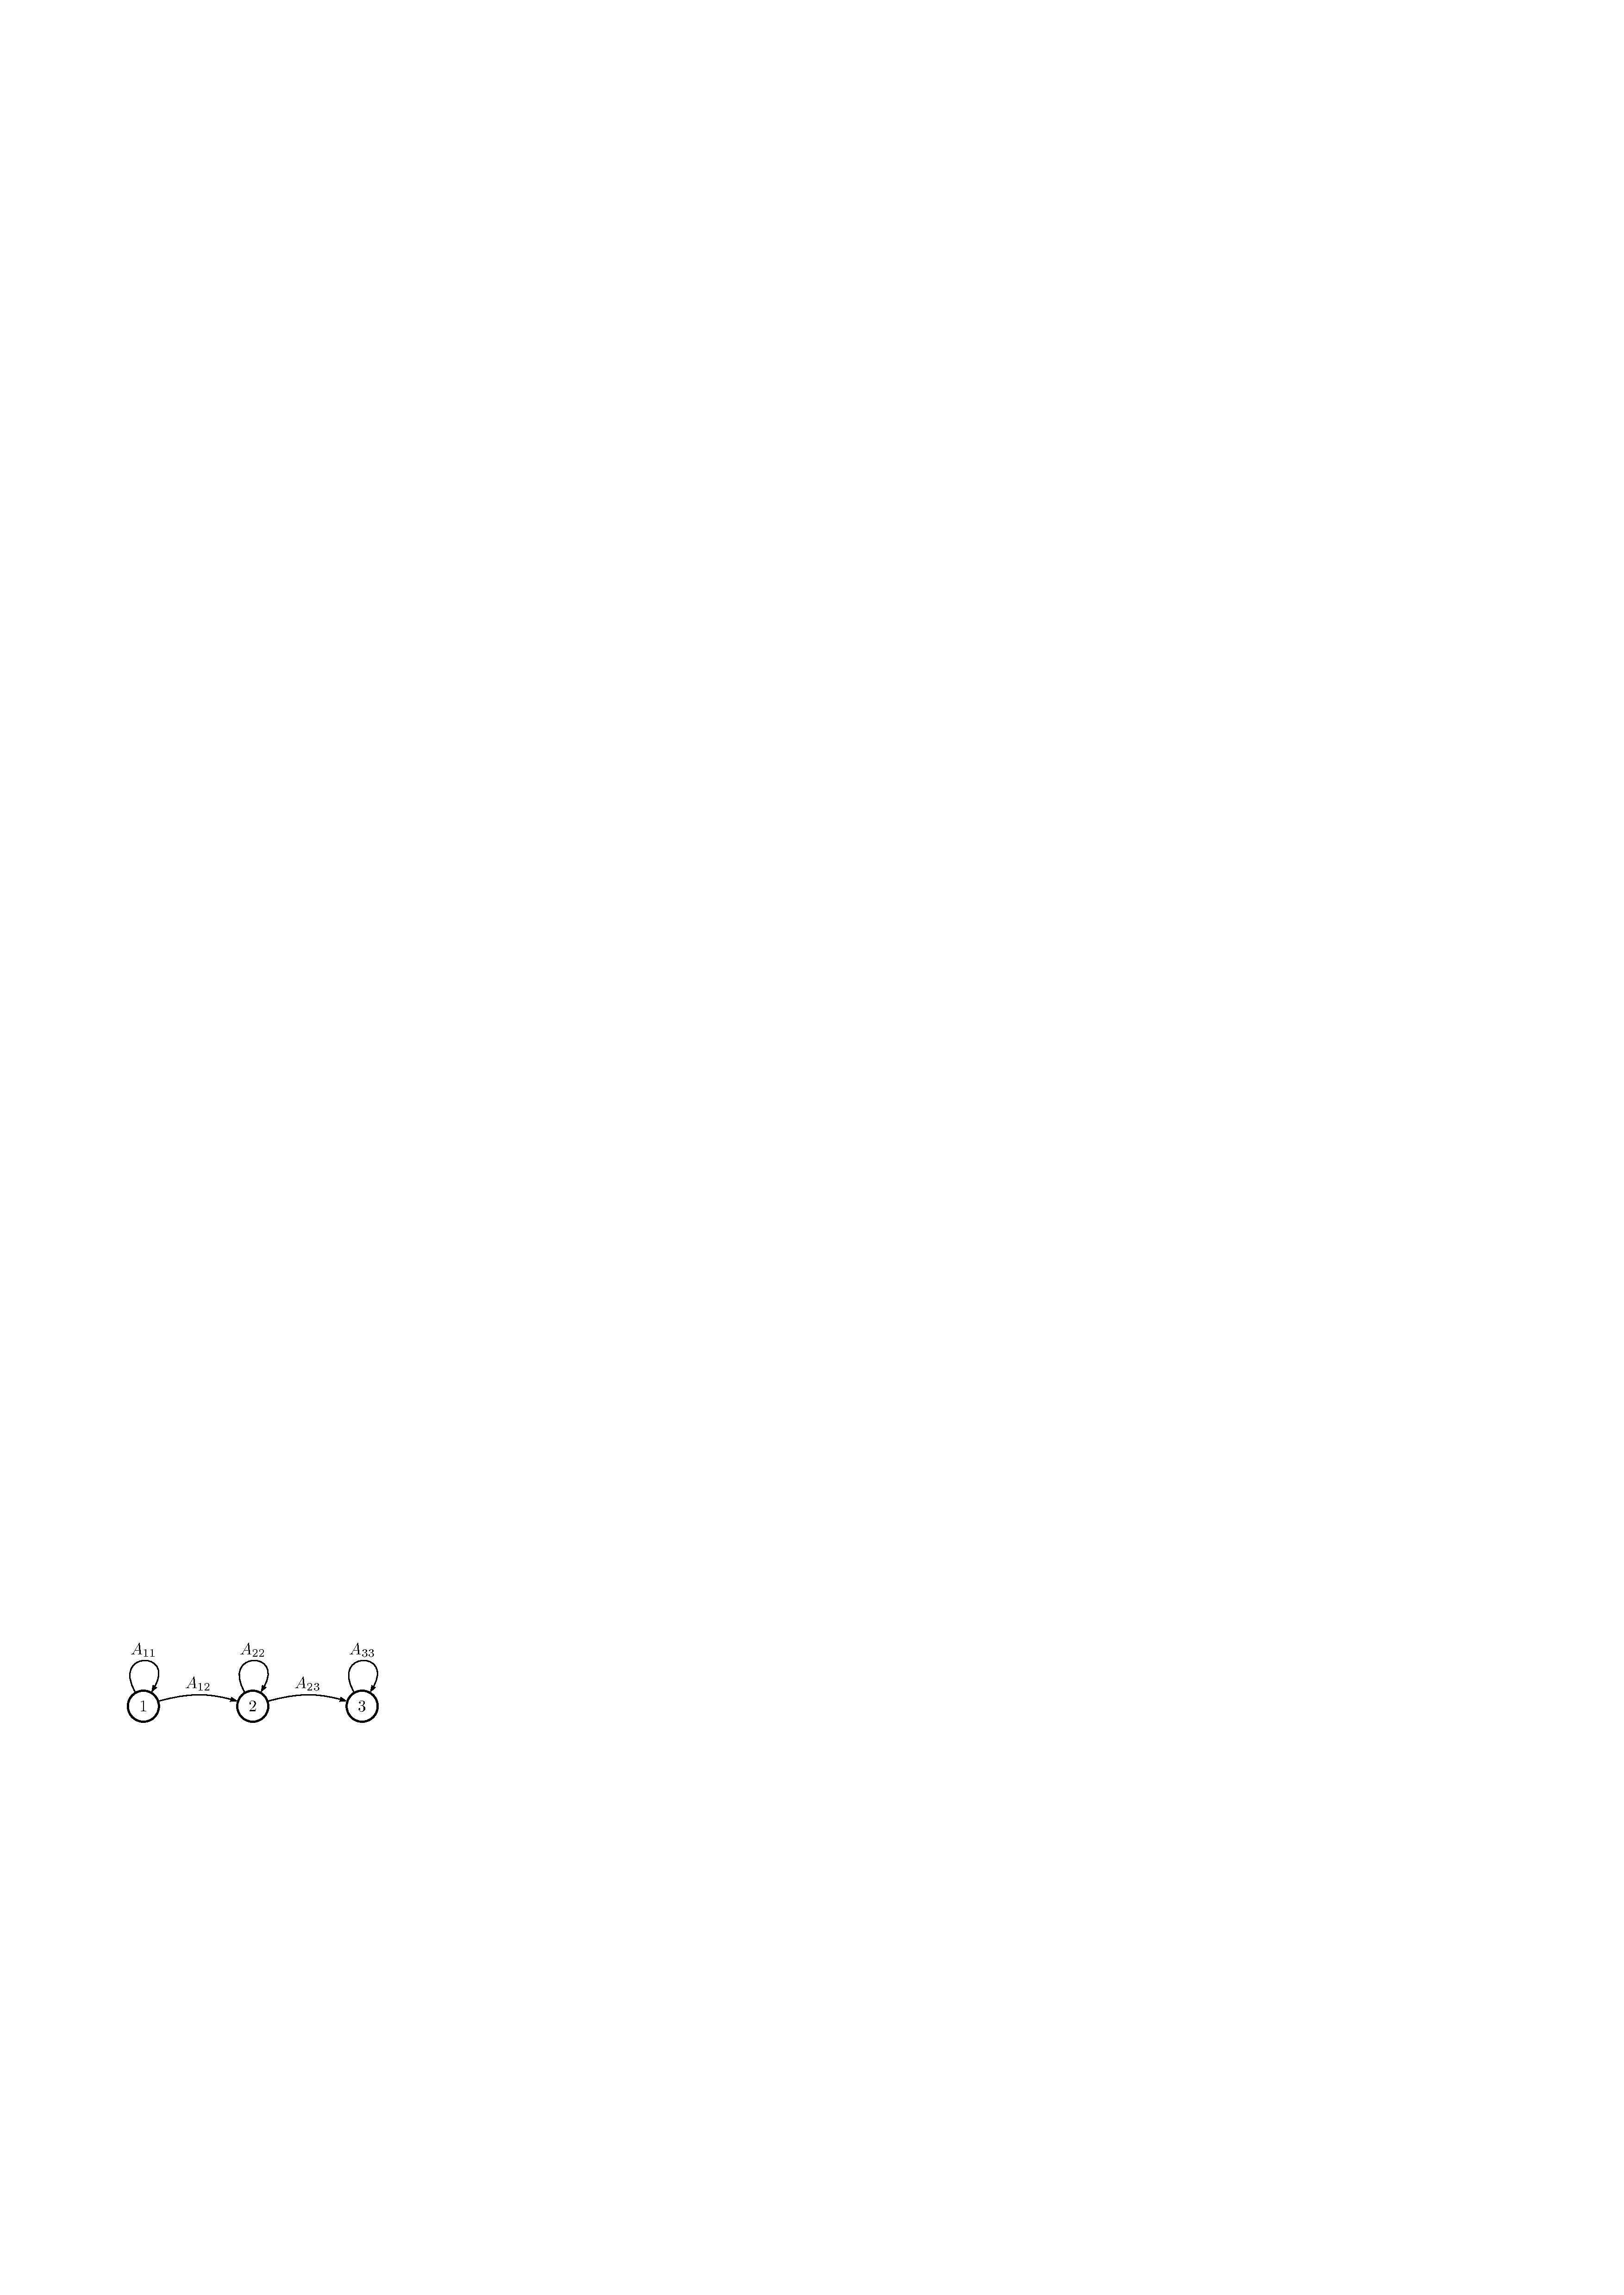
\includegraphics[width=40mm]{leftRightStateTrans}}
\caption{State transition diagrams for some simple Markov chains. Left: a 2-state chain. Right: a 3-state left-to-right chain.}
\end{figure}
\end{frame}

\begin{frame}{Hidden Markov Models (HMMs)}
%\begin{equation*}
    %p(x_{1:T}|z_{1:T}) = p(z_{1:T})p(x_{1:T}|z_{1:T})  = \left[ p(z_1) \prod_{t=2}^T p(z_t|z_{t-1}) \right] \left[ \prod_{t=2}^T p(x_t|z_t)\right]
%\end{equation*}

\begin{equation*}
    p(\bm{x}_{1:T}, \bm{z}_{1:T}) = p(\bm{z}_{1:T})p(\bm{x}_{1:T}|\bm{z}_{1:T})  = \left[ p(z_1) \prod_{t=2}^T p(z_t|z_{t-1}) \right] \left[ \prod_{t=1}^T p(\bm{x}_t|z_t)\right]
\end{equation*}

$z_t \rightarrow $ Hidden states taking one of K discrete values.\\
$x_t \rightarrow $ Observations taking values in space.

\begin{itemize}
    \item Discrete: $M$ observation symbols
    \begin{equation*}
        p(\bm{x}_t = l|z_t = k,\bm{\theta}) = B(k,l)
    \end{equation*}
    \item Continuous Gaussian:
    \begin{equation*}
        p(\bm{x}_t|z_t = k,\bm{\theta}) = N(\bm{x}_t|\bm{\mu}_k, \bm{\Sigma}_k)
    \end{equation*}
\end{itemize}
\end{frame}

\section{Inference in HMMs}
\begin{frame}{Types of inference problems for temporal models}
There are different kinds of inference, which we summarize below.
\begin{itemize}
    \item \textbf{Filtering:} computes the \textbf{belief state} $p(z_t|x_{1:t})$ online, or recursively, as the data streams in.
    \item \textbf{Smoothing}: computes $p(z_t|x_{1:T})$ offline, given all the evidence. 
    \item \textbf{Fixed lag smoothing} computes $p(z_{t-l}|x_{1:t})$, where $l > 0$ is \textbf{lag}.
    \item \textbf{Prediction} computes $p(z_{t+h}|x_{1:t})$, where $h > 0$ is called the \textbf{prediction horizon}. 
    \item \textbf{MAP estimation} computes $\text{arg}\max_{z_{1:T}} p(z_{1:T} |x_{1:T})$, which is a most probable state sequence (also known as \textbf{Viterbi decoding}). 
    \item \textbf{Posterior samples} $z_{1:T} \sim p(z_{1:T} |x_{1:T})$.
    \item \textbf{Probability of the evidence} computes the probability of the evidence, $p(x_{1:T}) = \sum_{z1:T} p(z_{1:T}, x_{1:T})$.
\end{itemize}
\end{frame}

\begin{frame}{The main kinds of inference for state-space models}
    \begin{figure}[h]
    \centering
    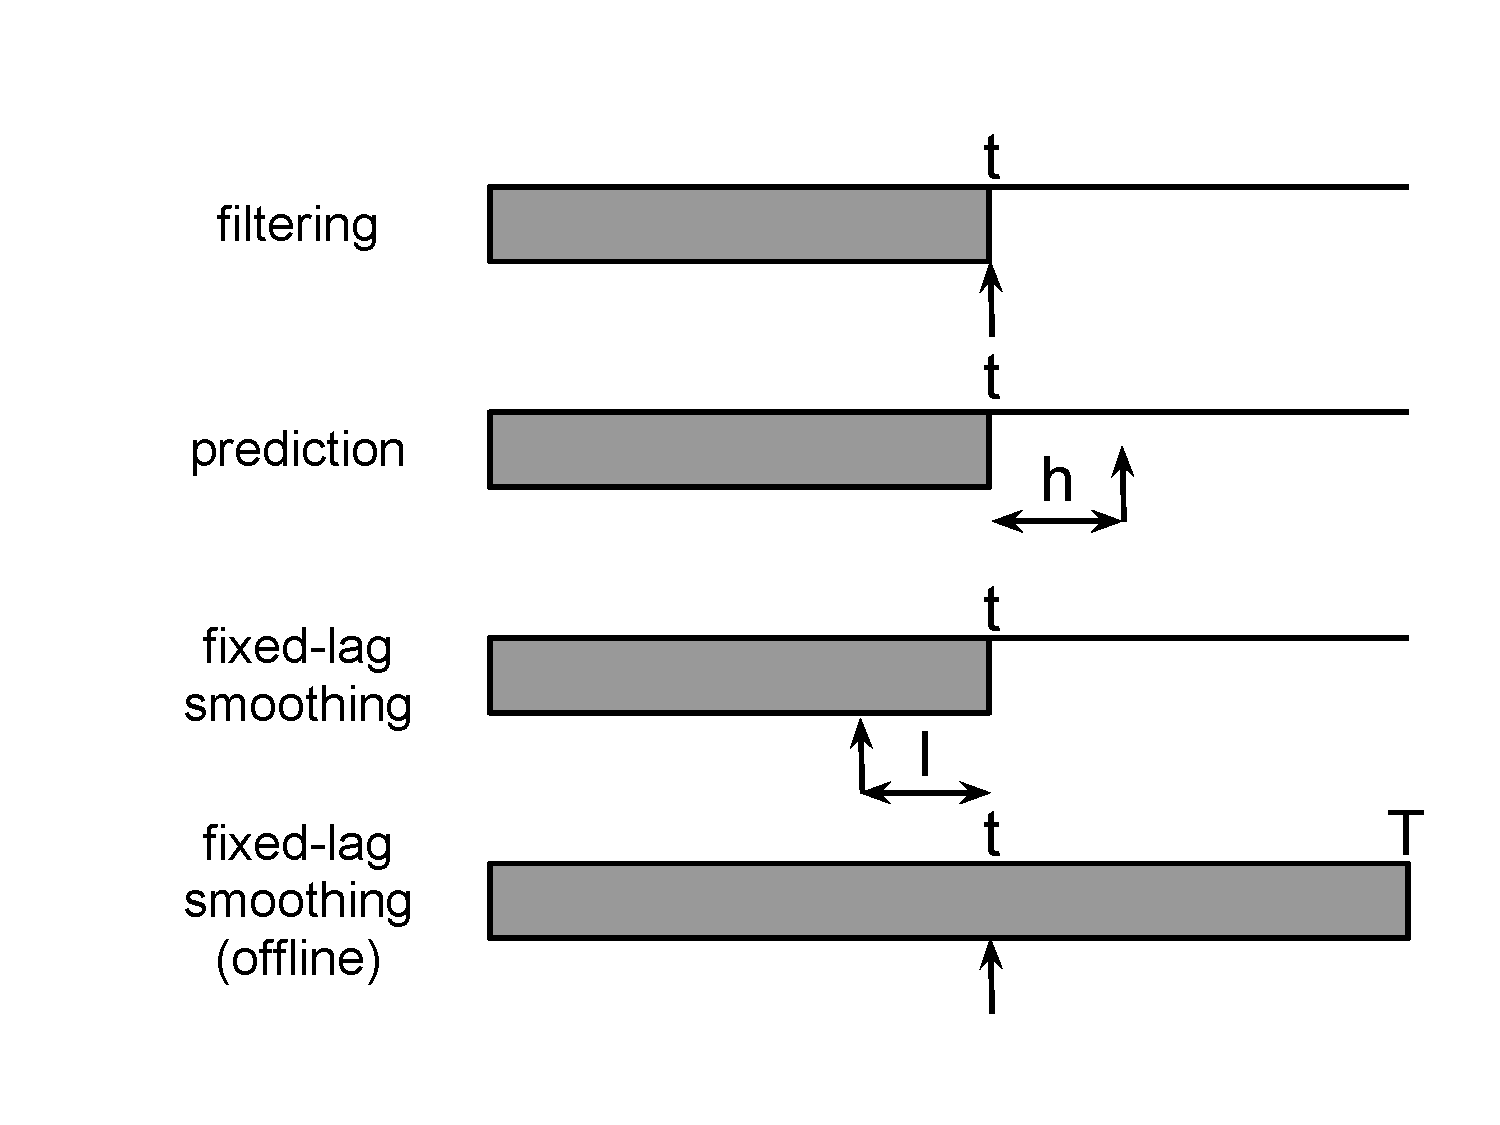
\includegraphics[width=0.4\textwidth]{dbn-inference-problems}
    \caption{The main kinds of inference for state-space models. The shaded region is the interval for which we have data. The arrow represents the time step at which we want to perform inference. $t$ is the current time, $T$ is the sequence length, $l$ is the lag and $h$ is the prediction horizon.}
    \end{figure}    
\end{frame}

%\begin{frame}{Forwards-backwards algorithm for chains}
%\\begin{itemize}
    %\\item Consider a 1d chain representing an HMM 
    %\\begin{equation*}
        %\p(\bm{z}, \bm{x}) = \prod_{t=1}^T p(z_t |z_{t-1})p(\bm{x}_t |z_t)
    %\\end{equation*}
    
    %\\item We first compute the filtered marginals in the forwards pass 
    %\\begin{equation*}
        %\\alpha_t(j) = p(z_t = j|\bm{x}_{1:t})
    %\\end{equation*}
    
    %\\item We then compute the smoothed marginals in the backwards pass
    %\\begin{equation*}
        %\\gamma_t(j) p(z_t =j|\bm{x}_{1:T})
    %\\end{equation*}
    
    %\\item As we explain below, this forwards-backwards algorithm takes $O(TK^2)$ time. It can also be applied to chain CRFs representing $p(\bm{z}_{1:T}|\bm{x}_{1:T})$.
    
    %\\item A simple modification yields the Viterbi algorithm which computes the most probable sequence of states (not the same as the sequence of most probable states):
    %\\begin{equation*}
        %\\bm{z}^* = \argmax p(\bm{z}|\bm{x}_{1:T})
    %\\end{equation*}
%\\end{itemize}
%\\end{frame}

\begin{frame}{Example: The occasionally dishonest casino}
\begin{figure}[h]
\centering
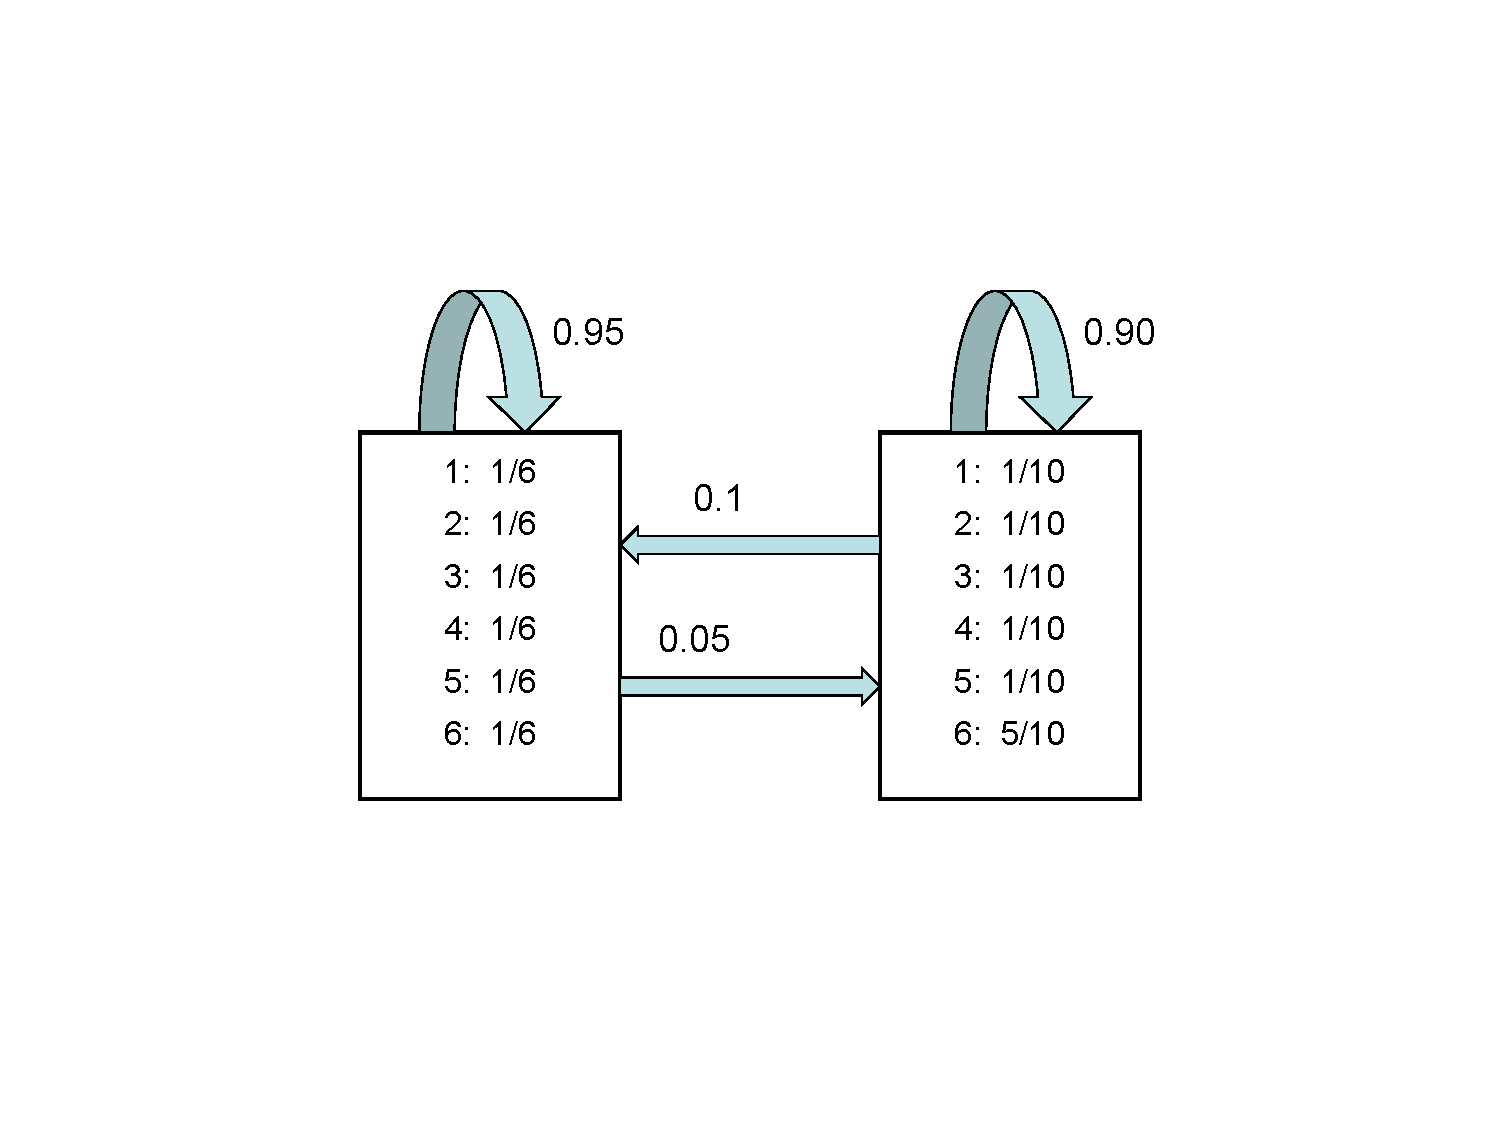
\includegraphics[width=0.3\textwidth]{casino}
\caption{An HMM for the occasionally dishonest casino. The blue arrows visualize the state transition diagram $A$. Based on (Durbin et al. 1998, p54).}
\end{figure}

$x_t\in \{1,2,...,6\}$ represents which dice face shows up, and $z_t$ represents the identity of the dice that is being used. Most of the time the casino uses a fair dice, $z = 1$, but occasionally it switches to a loaded dice, $z = 2$, for a short period.

\begin{itemize}
    \item Roll: \texttt{66415321616211523465321435663426165523423231514246415}.
    \item Dice: \texttt{LLLLLLLLLLLLLLFFFFFFLLLLLLLLLLLLLLFFFFFFFFFFFFFFFFFFL}.
\end{itemize}
\end{frame}

\begin{frame}{Filtering, smoothing, MAP}
\begin{figure}[h]
\centering     %%% not \center
\subfigure[]{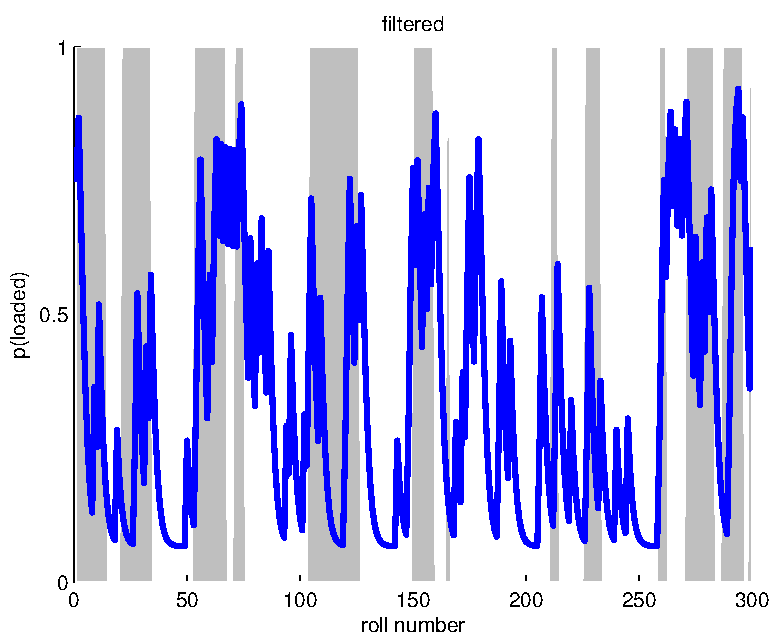
\includegraphics[width=20mm]{hmmCasinoFiltered}}
\subfigure[]{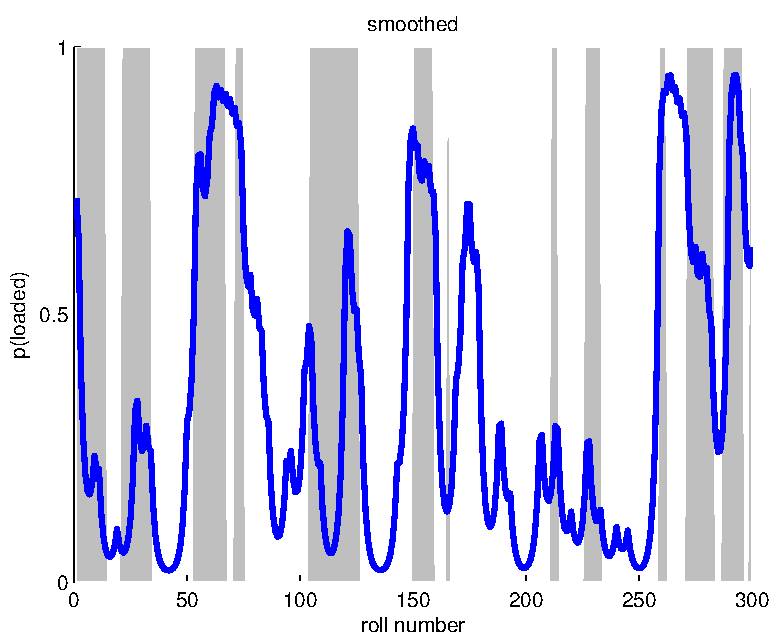
\includegraphics[width=20mm]{hmmCasinoSmoothed}}
\subfigure[]{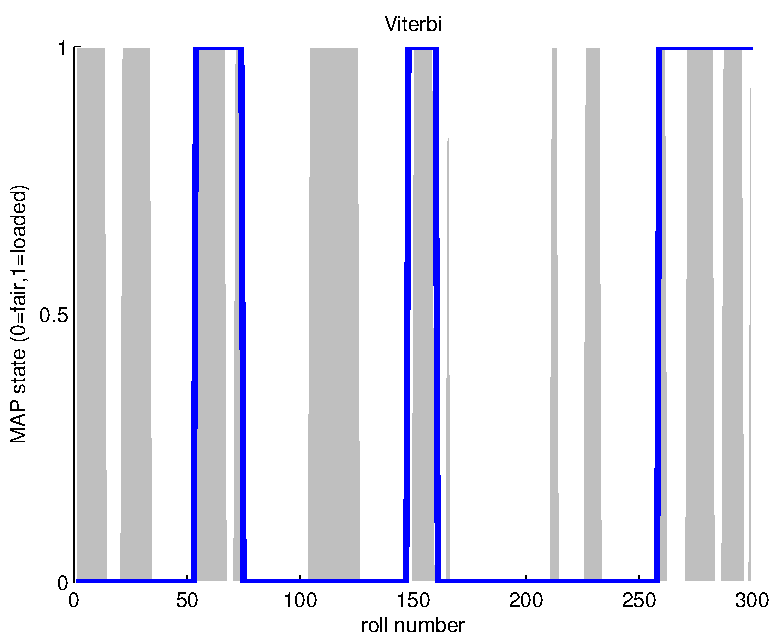
\includegraphics[width=20mm]{hmmCasinoViterbi}}
\caption{Inference in the dishonest casino. Vertical gray bars denote the samples that we generated using a loaded die. (a) Filtered estimate of probability of using a loaded dice. (b) Smoothed estimates. (c) MAP trajectory. Figure generated by \texttt{CasinoDemo}.}
\end{figure}

\begin{itemize}\footnotesize
    \item If we threshold the estimates at 0.5 and compare to the true sequence, we find that the filtered method makes 71 errors out of 300, the smoothed method makes 49/300, and the MAP path makes 60/300 errors.
    \item It is not surprising that smoothing makes fewer errors than Viterbi, since the optimal way to minimize bit-error rate is to threshold the posterior marginals.
    \item Nevertheless, for some applications, we may prefer the Viterbi decoding, to enforce consistency.
\end{itemize}
\end{frame}

\begin{frame}{Kalman filtering and smoothing}
\begin{figure}[h]
\centering     %%% not \center
\subfigure[]{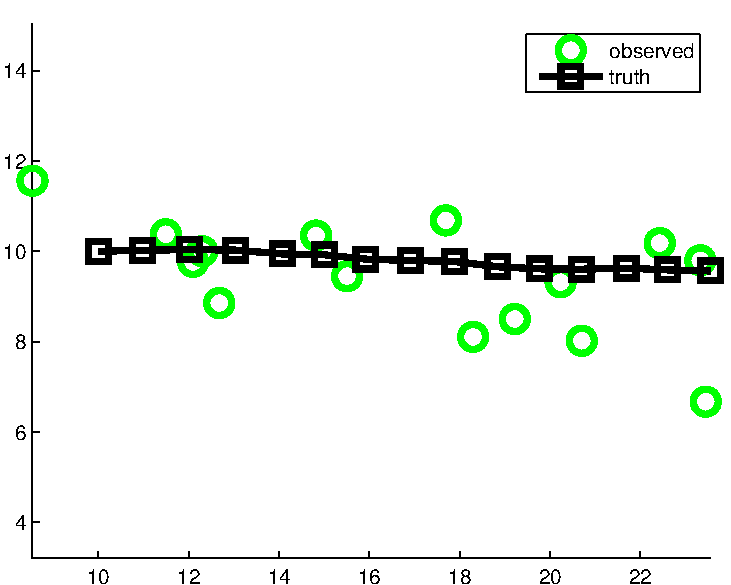
\includegraphics[width=20mm]{kalmanTrackingTruth}}
\subfigure[]{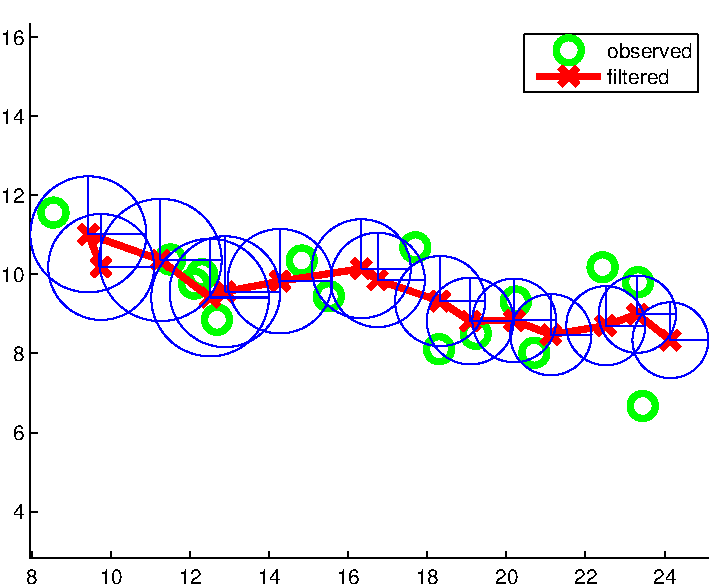
\includegraphics[width=20mm]{kalmanTrackingFiltered}}
\subfigure[]{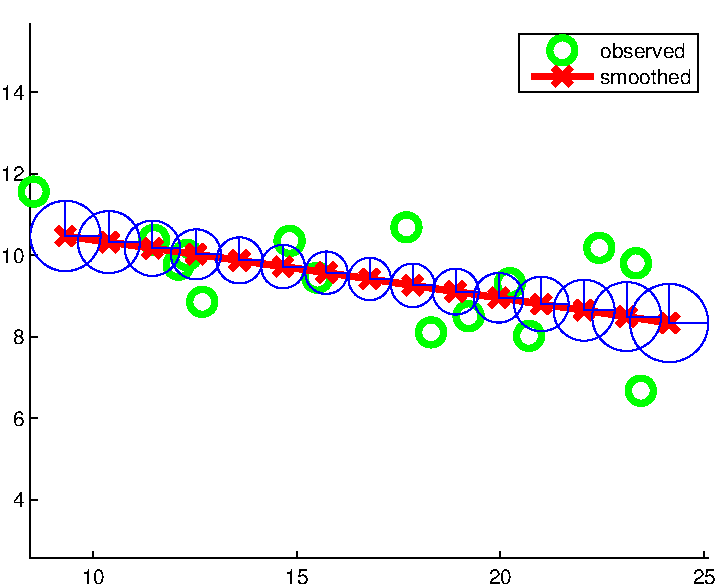
\includegraphics[width=20mm]{kalmanTrackingSmoothed}}
\caption{Illustration of Kalman filtering and smoothing. (a) Observations (green cirles) are generated by an object moving to the right (true location denoted by black squares). (b) Filtered estimated is shown by dotted red line. Red cross is the posterior mean, blue circles are 95\% confidence ellipses derived from the posterior covariance. For clarity, we only plot the ellipses every other time step. (c) Same as (b), but using offline Kalman smoothing. Figure generated by \texttt{kalmanTrackingDemo}.}
\end{figure}

\begin{itemize}
    \item Suppose $p(z, x)$ is a linear dynamical system subject to Gaussian noise, where $z\in \mathbb{R}^K$ and $x\in \mathbb{R}^D$.
    \item The analog of forwards-backwards is known as \textbf{Kalman filtering/ smoothing}.
\end{itemize}
\end{frame}

\begin{frame}{The forwards algorithm}
We now describe how to recursively compute the filtered marginals, $p(z_t|x_{1:t})$ in an HMM. 

\begin{itemize}
    \item We just apply Bayes rule sequentially to recursively update the belief state:
    \begin{equation*}
        \begin{split}
            \alpha_t(j) & = p(z_t = j|\bm{x}_{1:t}) = p(z_t = j|\bm{x}_t,\bm{x}_{1:t-1})\\
            & \ \propto \ p(\bm{x}_t|z_t = j, \cancel{\bm{x}_{1:t-1}})p(z_t = j|\bm{x}_{1:t-1})
        \end{split}
    \end{equation*}
    
    where $p(\bm{x}_t|z_t = j)$ is the likelihood and the prior is the one-step-ahead predictive density
    \begin{equation*}
        p(z_t = j|\bm{x}_{1:t-1}) = \sum_i p(z_t=j|z_{t-1}=i)\alpha_{t-1}(i)
    \end{equation*}
    
    \item This is called the \textbf{predict-update cycle}.
    \item In matrix-vector notation, we can write the update in the following simple form:
    \begin{equation*}
        \bm{\alpha}_t \ \propto \ \bm{\psi}_t \odot (\bm{\Psi}^T \bm{\alpha}_{t-1})
    \end{equation*}
    
    \item The base case is $\bm{\alpha}_1 \ \propto \ \bm{\psi}_1 \odot \bm{\pi}$. 
\end{itemize}
\end{frame}

\begin{frame}{The backwards algorithm}
\begin{itemize}
    \item The key decomposition relies on the fact that we can break the chain into two parts, the past and the future, by conditioning on $z_t$:
    \begin{equation*}
        \begin{split}
            p(z_t = j|\bm{x}_{1:T}) &  \propto  p(z_t = j,\bm{x}_{t+1:T}|\bm{x}_{1:t})\\
            & \propto  p(z_t = j|x_{1:t})p(x_{t+1:T}|z_t = j, \cancel{x_{1:t}})
        \end{split}
    \end{equation*}
    
    We define
    \begin{equation*}
        \begin{split}
            \beta_t(j) & = p(\bm{x}_{t+1:T}|z_t =j) \\
            \gamma_t(j) & = p(z_t = j|x_{1:T})
        \end{split}
    \end{equation*}
    %as the conditional likelihood of future evidence given that the hidden state at time $t$ is $j$.
    
    From above equation, we have
    \begin{equation*}
         \gamma_t(j) = \alpha_t(j)\beta_t(j)
    \end{equation*}
    
    \item We now derive a recursive update for $\beta_t$. (It is also possible to directly update $\gamma_t$.)
\end{itemize}
\end{frame}

\begin{frame}{The backwards algorithm}
\begin{itemize}
    \item Working right to left, we have
    \begin{equation*}
        \begin{split}
            \beta_{t-1}(i) & = p(\bm{x}_{t:T}|z_{t-1}=i)\\
            & = \sum_j p(z_t =j,\bm{x}_t,\bm{x}_{t+1:T}|z_{t-1} =i)\\
            & = \sum_j p(\bm{x}_{t+1:T} |z_t =j,\cancel{\bm{x}_t},\cancel{z_{t-1} =i})p(z_t =j,\bm{x}_t |z_{t-1} =i)\\
            & = \sum_j p(\bm{x}_{t+1:T} |z_t =j) p(\bm{x}_t|z_t=j,\cancel{z_{t-1}=j})p(z_t =j,\bm{x}_t |z_{t-1} =i)\\
            &  = \sum_j\beta_t(j)\phi_t(j)\phi(i,j)
        \end{split}
    \end{equation*}
    
    \item We can write the resulting equation in matrix-vector form as
    \begin{equation*}
        \bm{\beta}_{t-1} = \bm{\Psi}(\bm{\psi}_t \odot \bm{\beta}_t)
    \end{equation*}
    
    \item The base case is
    \begin{equation*}
        \beta_T(i) = p(\bm{x}_{T+1:T}|z_T = i) = p(\emptyset|z_T = i) = 1
    \end{equation*}
    which is the probability of a non-event.
\end{itemize}
\end{frame}

\begin{frame}{The Viterbi algorithm}
\begin{figure}[h]
\centering
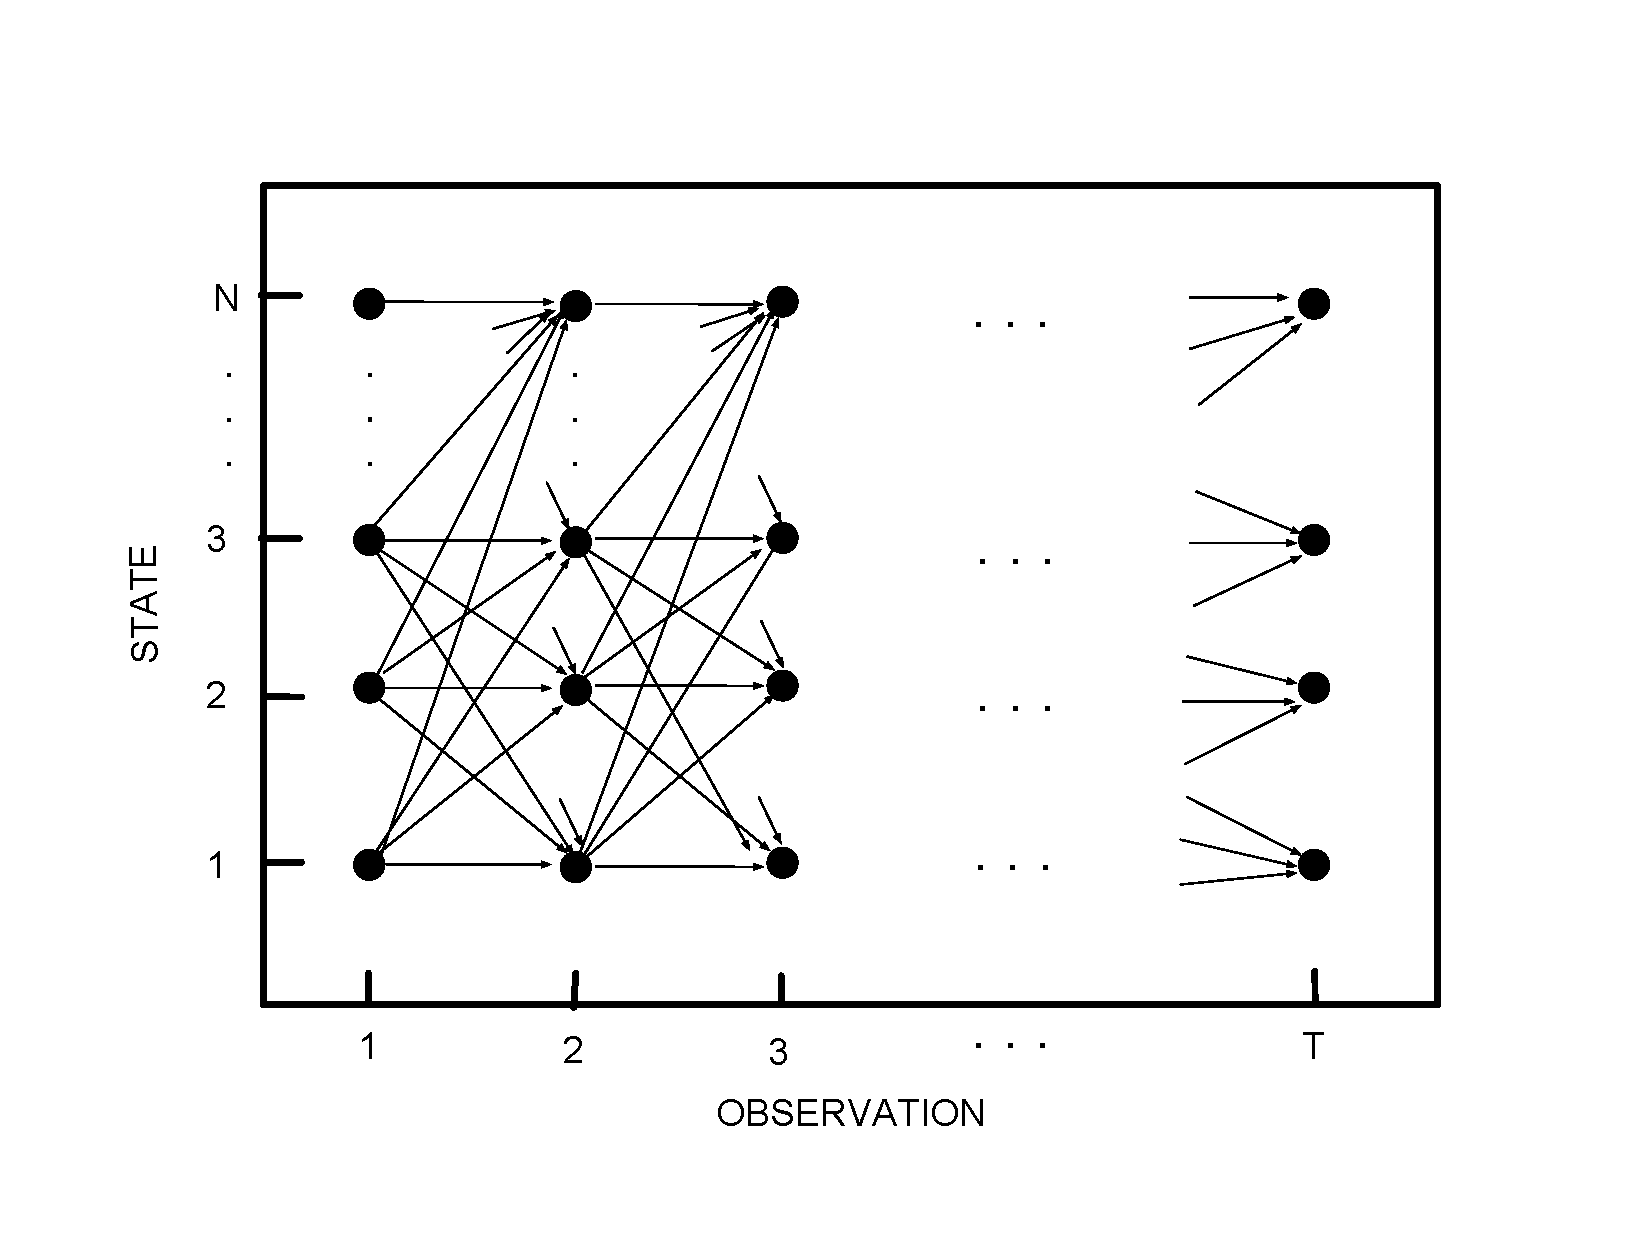
\includegraphics[width=0.3\textwidth]{markovTrellis}
\caption{The trellis of states vs time for a Markov chain. Based on (Rabiner 1989).}
\end{figure}

\begin{itemize}\footnotesize
    \item  The Viterbi algorithm can be used to compute the most probable sequence of states in a chain-structured graphical model, i.e.,
    \begin{equation*}
        \bm{z}^* = \argmax p(\bm{z}_{1:T} |\bm{x}_{1:T} )
    \end{equation*}
    
    \item  This is equivalent to computing a shortest path through the \textbf{trellis diagram} where the nodes are possible states at each time step, and the node and edge weights are log probabilities. That is, the weight of a path $z_1,z_2,...,z_T$ is given by
    \begin{equation*}
        \log \pi_1(z_1) + \log \phi_1(z_1) +  \sum_{t=2}^T [\log \phi(z_{t-1}, z_t ) + \log \phi_t (z_t )]
    \end{equation*}
\end{itemize}
\end{frame}

\begin{frame}
\begin{itemize}\footnotesize
    \item We already have 
    \begin{equation*}
        p(\bm{x}_{1:T}, \bm{z}_{1:T}) = p(\bm{z}_{1:T})p(\bm{x}_{1:T}|\bm{z}_{1:T})  = \left[ p(z_1) \prod_{t=2}^T p(z_t|z_{t-1}) \right] \left[ \prod_{t=1}^T p(\bm{x}_t|z_t)\right]
    \end{equation*}
    
    \begin{equation*}
        \hat{z} = \argmax_z p(z|x) = \argmax_z = p(z, x)
    \end{equation*}
    
    \item Equivalent to minimizing negative log-probability:
    \begin{equation*}
        \begin{split}
             \phi_1(z_1) & = - \log p(z_1) - \log p(x_1|z_1)\\
             \phi_t(z_t) & = - \log p(x_t|z_t) \\
             \psi_t(z_{t-1}, z_t) & = - \log p(z_t|z_{t - 1})
        \end{split}
    \end{equation*}
    
    \begin{equation*}
        \hat{z} = \argmin_z \phi_1(z_1) +  \sum_{t=2}^T [\psi_t(z_{t-1}, z_t) + \phi_t(z_t)]
    \end{equation*}    
\end{itemize}
\end{frame}

\begin{frame}{MAP vs MPM}
\begin{itemize}
    \item The (jointly) most probable sequence of states is not necessarily the same as the sequence of (marginally) most probable states.
    \item In Viterbi, when we estimate $z_t$, we ``max out" the other variables:
    \begin{equation*}
        z_t^* =\text{arg}\max_{z_t} \max_{\bm{z}_{1:t -1} ,\bm{z}_{t +1:T}} p(\bm{z}_{1:t -1},z_t,\bm{z}_{t+1:T}|\bm{x}_{1:T})
    \end{equation*}
    
    whereas we when we use forwards-backwards, we sum out the other variables to get a maximum posterior marginal (MPM):
    \begin{equation*}
        \hat{z}_t =\argmax_{z_t} \max_{\bm{z}_{1:t -1} ,\bm{z}_{t +1:T}} p(\bm{z}_{1:t -1},z_t,\bm{z}_{t+1:T}|\bm{x}_{1:T})
    \end{equation*}
    
    \item The sequence of MPMs may not be equal to the joint MAP sequence, e.g., ``wreck a nice beach" might be the MPM interpretation of a series of acoustic waveforms, but the MAP sequence is more likely to be ``recognize speech".
\end{itemize}
\end{frame}

\begin{frame}{Details of the algorithm}
We implement Viterbi by replacing the sum-operator in forwards-backwards with a max-operator. The former is called the \textbf{sum-product}, and the latter the \textbf{max-product} algorithm.\bigskip
\begin{itemize}
    \item Define the probability of ending up in state $j$ at time $t$, given that we take the most probable path:
    \begin{equation*}
        \delta_t(j) =  \max_{z_1,...,z_{t -1}} p(\bm{z}_{1:t-1}, z_{t} = j|\bm{x}_{1:t}) 
    \end{equation*}
    
    \item The most probable path to state $j$ at time $t$ must consist of the most probable path to some other state $i$ at time $t - 1$, followed by a transition from $i$ to $j$.
    \begin{equation*}
        \delta_t(j) = \max_i\delta_{t-1}(i)\psi(i,j)\phi_t(j)
    \end{equation*}

    \item We also keep track of the most likely previous state, for each possible state that we end up in:
    \begin{equation*}
        a_t(j) = \text{arg}\max\delta_{t-1}(i)\psi(i,j)\psi_t(j)
    \end{equation*}
    $a_t(j)$ tells us the most likely previous state on the most probable path to $z_t = j$. 
initialize by setting
\end{itemize}
\end{frame}

\begin{frame}
\begin{itemize}
    \item We initialize by setting
    \begin{equation*}
        \delta_1(j) = \pi_j\phi_1(j)
    \end{equation*}
    \item and we terminate by computing the most probable final state $z_T^∗$:
    \begin{equation*}
        z_T^∗ = \argmax_i \delta_T(i)
    \end{equation*}
    \item We can then compute the most probable sequence of states using \textbf{traceback}:
    \begin{equation*}
        z_t^* = a_{t+1} (z_{t+1}^*)
    \end{equation*}
\end{itemize}
\end{frame}

\section{Learning for HMMs}
\begin{frame}{Learning for HMMs}
We now discuss how to estimate the parameters $ \bm{\theta}= (\bm{\pi},\bm{A},\bm{B})$, where
\begin{itemize}
    \item $\pi(i) = p(z_1 = i)$ is the initial state distribution.
    \item $A(i,j) = p(z_t = j|z_{t-1} = i)$ is the transition matrix.
    \item $\bm{B}$ are the parameters of the class-conditional densities $p(\bm{x}_t|z_t = j)$.
\end{itemize}
\end{frame}

\begin{frame}{Training with fully observed data}
\begin{itemize}
    \item If we observe the hidden state sequences, we can compute the MLEs for $\bm{A}$ and $\bm{\pi}$.
    \item The details on how to estimate $\bm{B}$ depend on the form of the observation model.
    \item  For example, if each state has a multinoulli distribution with parameters $B_{jl} = p(X_t = l|z_t = j)$
    \begin{equation*}
        \hat{B}_{jl} = \frac{N_{jl}^X}{N_j}, \quad N_{jl}^X = \sum_{i=1}^N \sum_{t=1}^{T_i}\mathbb{I}(z_{i,t} = j, x_{i,t} = l)
    \end{equation*}
    \item This result is quite intuitive: we simply add up the number of times we are in state $j$ and we see a symbol $l$, and divide by the number of times we are in state $j$.
\end{itemize}
\end{frame}

\begin{frame}{Training with unobserved data}
If the $z_t$ variables are not observed, we apply the EM algorithm to HMMs, also known as the \textbf{Baum-Welch} algorithm.\bigskip

\begin{itemize}\footnotesize
    \item E step: the expected complete data log likelihood
    \begin{equation*}
        \begin{split}
            Q(\bm{\theta},\bm{\theta}^{\text{old}}) = & \sum_{k=1}^K E[N_k^1] \log\pi_k + \sum_{j=1}^K\sum_{k=1}^K E[N_{jk}]\log A_{jk}\\
            & + \sum_{i=1}^T\sum_{t=1}^{T_i}\sum_{k=1}^K p(z_t = k | \bm{x}_i,\bm{\theta}^{\text{old}})\log p(\bm{x}_{i,t}|\bm{\phi}_k)
        \end{split}
    \end{equation*}
    where the expected counts are given by
    \begin{equation*}
        \begin{split}
            E[N_k^1] = & \sum_{i=1}^N p(z_{i1} = k | \bm{x}_i,\bm{\theta}^{\text{old}})\\
            E[N_{jk}] = & \sum_{i=1}^T\sum_{t=2}^{T_i}p(z_{i,t-1} = j, z_{i,t} = k | \bm{x}_i,\bm{\theta}^{\text{old}})\\
            E[N_j] = & \sum_{i=1}^T\sum_{t=1}^{T_i}p(z_{i,t} = j | \bm{x}_i,\bm{\theta}^{\text{old}})\\
        \end{split}
    \end{equation*}
\end{itemize}
\end{frame}  

\begin{frame}{Training with unobserved data (cont'd)}
\begin{itemize}
    \item M step for $\bm{A}$ and $\pi$ is to just normalize the expected counts:
      \begin{equation*}
          \hat{A}_{jk}  = \frac{E[N_{jk}]}{\sum_{k'}E[N_{jk'}]}, \ \hat{\pi}_k = \frac{E[N_k^1]}{N}
      \end{equation*}
    \item This result is quite intuitive: we simply add up the expected number of transitions from $j$ to $k$, and divide by the expected number of times we transition from $j$ to anything else.
\end{itemize}
\end{frame}
\end{document}
